\documentclass[serif, pdf]{beamer}

%   Theme
\usetheme{Warsaw}

%   Packages
\usepackage{xcolor}
\usepackage{tikz}
\usepackage{multimedia}
\usepackage{lmodern}
\usepackage{scrextend}
\usepackage{subcaption}
\usepackage[normalem]{ulem}
%\usepackage{media9}
%\usepackage{movie15}

\usepackage{makecell}
\setcellgapes{4pt}

\usepackage{caption}
\captionsetup[figure]{labelformat=empty}

\setbeamerfont{caption}{size=\scriptsize}

\usecolortheme{beaver}

%   Metadata
\title[MOD]{Generation And Simulation Of Manufacturable 2D Soft Bodies}
\date{8 May 2020}
\author[Naud\'e Conradie]{Naud\'e Conradie\\{\small Supervisor: Dr MP Venter}}
\institute[]{Department of Mechanical and Mechatronic Engineering, Stellenbosch University}

%   Colour definitions
\definecolor{colour1}{RGB}{96, 34, 59}
\definecolor{colour2}{RGB}{140, 151, 154}
\setbeamercolor{structure}{fg=colour1,bg=colour2}
\setbeamercolor{title}{fg=white,bg=colour2}
\setbeamercolor{author in head/foot}{fg=colour1}

%   Beamer template settings
\setbeamertemplate{itemize item}{\color{black}$\bullet$}
\setbeamertemplate{itemize subitem}{\color{black}$-$}
\setbeamertemplate{caption}{\raggedright\insertcaption\par}

%   Footer settings
\expandafter\def\expandafter\insertshorttitle\expandafter{%
  \insertshorttitle\hfill%
  \hspace{30mm}\insertframenumber\,/\,\inserttotalframenumber}

\beamertemplatenavigationsymbolsempty

\begin{document}

%   Title Slide-------------------------------------------------%

\begin{frame}
  \begin{center}
    \vspace{0.1cm}
    \includegraphics[scale=0.25]{USlogo.pdf}
  \end{center}
  \titlepage
\end{frame}

%   Overview----------------------------------------------------%

\changefontsizes{13pt}
\begin{frame}
    \frametitle{Presentation Overview}
    \begin{itemize}
        \item<1-> Project scope
        \item<2-> Objectives
        \item<3-> Methodology
        \item<4-> Upcoming Work
    \end{itemize}
\end{frame}

%   Project Scope-----------------------------------------%

\begin{frame}
    \frametitle{Project Scope}
    \begin{itemize}
        \item<1-> Automate the generation and simulation of 2D soft bodies
        \changefontsizes{11pt}
        \begin{itemize}
            \item<2-> Generate 2D bodies built from smaller building blocks with specific deformations
            \item<3-> Non-linear FEM with hyper-elastic material models
            \item<4-> Evaluate the bodies and building blocks according to predefined goals
        \end{itemize}
    \end{itemize}
\end{frame}

%   Objectives-----------------------------------------%

\begin{frame}
    \frametitle{Objectives}
    \begin{itemize}
        \item<1-> Automation for future use and development
        \item<2-> Generation of soft bodies built from generated smaller units
        \item<3-> Selection of best models according to selected metrics
        \item<4-> Accurate modelling of real-world materials
        \item<5-> Computationally efficient manner
        \item<6-> Limitations
        \changefontsizes{11pt}
        \begin{itemize}
            \item<7-> Two dimensions
            \item<8-> Pre-existing material models
        \end{itemize}
    \end{itemize}
\end{frame}

%   Software----------------------------------------------------%

\changefontsizes{13pt}
\begin{frame}
    \frametitle{Software}
    \begin{itemize}
        \item<1-> LS-Dyna
        \changefontsizes{11pt}
        \begin{itemize}
            \item<2-> License expired
        \end{itemize}
        \item<3-> Siemens NX 12
        \changefontsizes{11pt}
        \begin{itemize}
            \item<4-> Unnecessary
        \end{itemize}
        \item<3-> MSC Marc Mentat
        \changefontsizes{11pt}
        \begin{itemize}
            \item<5-> Python
        \end{itemize}
    \end{itemize}
\end{frame}

%   Methodology-----------------------------------------%

\begin{frame}
    \frametitle{Methodology}
    \begin{itemize}
        \item<1-> Generate grid of square elements
        \item<2-> Random internal elements are removed
        \item<3-> Simulation is evaluated
        \begin{itemize}
            \item<4-> Maximum stress
            \item<5-> Boundary energy
            \begin{itemize}
            	\item<6-> \begin{equation*}
            	E_{b}=\sum_{i=1}^{n_{n}}d_{i}\times F_{i}
            	\end{equation*}
            	\item<6-> If i is a boundary node
            \end{itemize}
        \end{itemize}
    \end{itemize}
\end{frame}

%   Methodology-----------------------------------------%

\begin{frame}
    \frametitle{Methodology (cont.)}
    \begin{figure}[h]       
    	\mbox{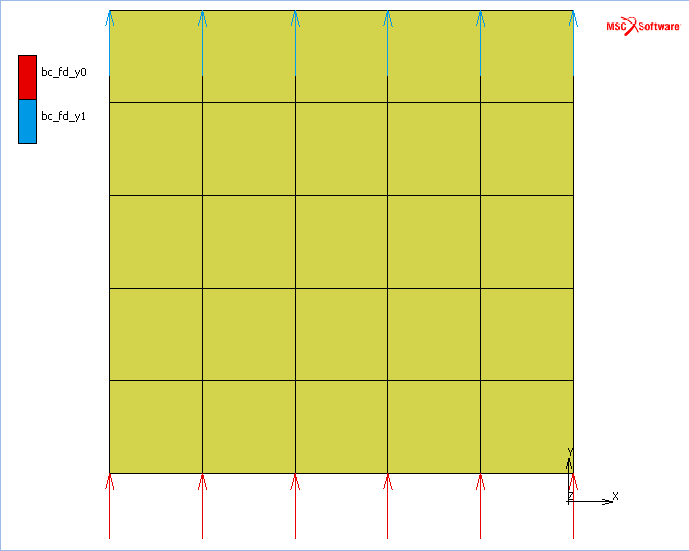
\includegraphics[width=0.3\linewidth]{Example-Template.png}}   
    	\hspace{3px}
    	\mbox{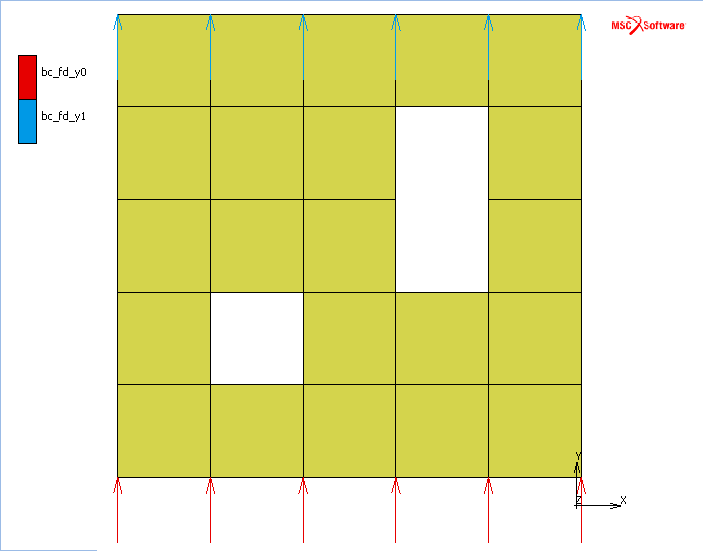
\includegraphics[width=0.3\linewidth]{Example-Model.png}}
    	\hspace{3px}
    	\mbox{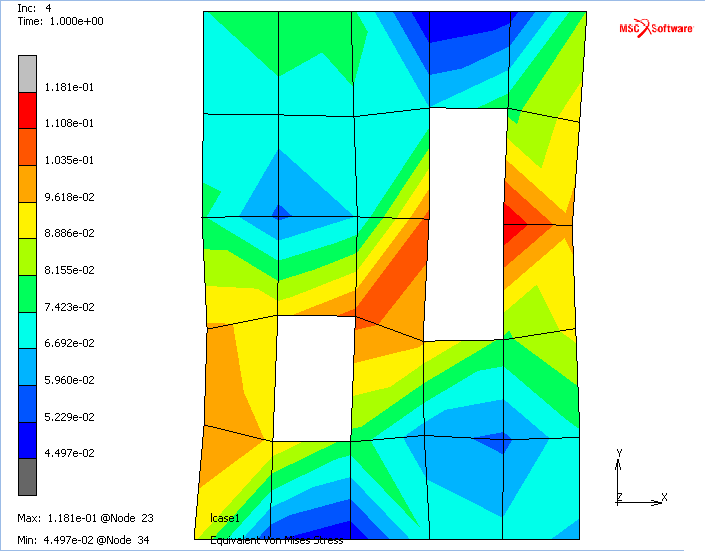
\includegraphics[width=0.3\linewidth]{Example-Model-Results.png}}
	\end{figure}
\end{frame}

%   Methodology-----------------------------------------%

\begin{frame}
    \frametitle{Methodology (cont.)}
    \begin{center}
        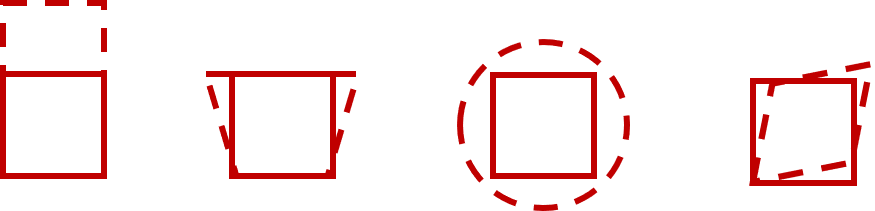
\includegraphics[width=1\linewidth]{Example-Shapes.png}
    \end{center}
\end{frame}

%   File Hierarchy-----------------------------------------%

\begin{frame}
    \frametitle{File Hierarchy}
	\begin{center}
        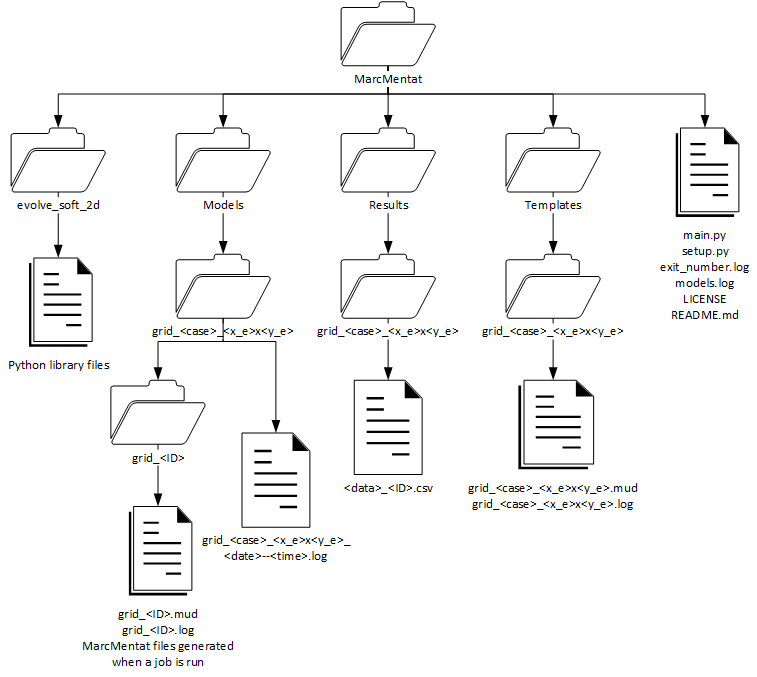
\includegraphics[width=0.8\linewidth]{File-Hierarchy.png}
    \end{center}
\end{frame}

%   Material Models------------------------------------------%

\begin{frame}
    \frametitle{Material Models}
    \begin{itemize}
        \item<1-> Material testing of Mold Star 15 and possibly other materials
        \changefontsizes{11pt}
        \begin{itemize}
            \item<2-> Tensile testing
            \changefontsizes{11pt}
        	\begin{itemize}
            	\item<3-> Long travel extensometer
            	\item<4-> DIC
            \end{itemize}
            \item<5-> Compression testing
            \changefontsizes{11pt}
        	\begin{itemize}
            	\item<6-> DIC
            \end{itemize}
        \end{itemize}
        \item<7-> Ogden material model
        \changefontsizes{11pt}
        \begin{itemize}
            \item<8-> \begin{equation*}
            W_{1}\left(\lambda_{1},\lambda_{2},\lambda_{3}\right)=\sum_{i=1}^{N}\frac{\mu_{i}}{\alpha_{i}}\left(\lambda_{1}^{\alpha_{i}}+\lambda_{2}^{\alpha_{i}}+\lambda_{3}^{\alpha_{i}}-3\right)
            \end{equation*}
        \end{itemize}
    \end{itemize}
\end{frame}

%   Upcoming work------------------------------------------%

\begin{frame}
    \frametitle{Upcoming Work}
    \begin{itemize}
        \item<1-> Select best performing units
        \item<2-> Build bodies from units
		\begin{itemize}
            \item<3-> Generative design
            \begin{itemize}
            	\item<4-> L-systems
            	\item<5-> CPPNs
            \end{itemize}
        \end{itemize}
    \end{itemize}
\end{frame}

%   Questions---------------------------------------------------%

\begin{frame}
    \begin{center}
        \huge Questions?
    \end{center}
\end{frame}

\end{document}
